\graphicspath{{./Sterownik/images}}

\chapter{Sterownik kontrolera klinostatu}

Jako kontroler klinostatu rozumie się jednostkę odpowiadającą za bezpośrednie sterowanie silnikami oraz pompą wody. Jest to część systemu z którą operator urządzenia nie wchodzi bezpośrednio w interakcję, a sterowana jest ona pośrednio przez interfejs użytkownika aplikacji, poprzez system wbudowanych komend. Kontroler stanowi całkowicie odrębne urządzenie niż komputer z którego sterowany jest klinostat, natomiast nie jest ono w stanie działać samodzielnie bez kontaktu z rdzeniem systemu. Sterownik wymagał implementacji w niskopoziomowym języku programowania, ze względu na wybór platformy z mikroprocesorem typu AVR. Wybrany został w tym celu język C++. W dalszej części pracy do programu kontrolera klinostatu będzie 
\section{Założenia funkcjonalne sterownika}

Poniżej wymieniono funkcjonalności oraz założenia jakie musiał spełniać sterownik kontrolera klinostatu:

\begin{itemize}
	
	\item Sterowanie silników powinno być całkowicie niezależne od reszty funkcjonalności programu. Oznacza to iż odbieranie oraz wysyłanie danych przez port szeregowy powinno odbywać się równolegle z operacjami obsługującymi układ napędowy.
	\item Silniki domyślnie powinny uruchamiać się oraz zatrzymywać ze stałym przyspieszeniem tzn. prędkości obrotowe powinny zmieniać się liniowo podczas rozruchu oraz zatrzymania klinostatu.
	\item Sterownik powinien również niezależnie śledzić czas, który upłynął od rozpoczecia programu. Z pomocą odmierzania czasu obliczana jest objętość wody wpompowanej do komory środowiskowej.

\end{itemize}

COŚ TUTAJ JESZCZE DODAĆ, NA RAZIE PLACEHOLDER.


\section{Platforma}

Wspomniano wcześniej iż w skład elektroniki klinostatu wchodzi płytka rozwojowa Arduino Leonardo. Jednostka mikrokontrolera (ang. \angver{microcontroller unit}, MCU) znajdująca się na tym rodzaju płytki to ATmega32U4 produkowana przez firmę Atmel. Jest to 8-bitowy MCU typu AVR, który w przypadku płytki Arduino taktowany jest za pomocą zewnętrznego oscylatora kwarcowego o częstotliwości \SI{16}{MHz}. Platforma ta została wybrana na etapie projektowym, kierując się jej dostępnością, popularnością, ceną oraz parametrami. Platformy Arduino w odniesieniu do samodzielnych kontrolerów AVR oferują znacznie prostsze metody programowania poprzez udostępnienie wielu bibliotek, które interfejsują z samymi rejestrami mikrokontrolera. Powoduje to efektywnie programowanie wyższego poziomu. Minusem takiego podejścia jest konieczność umieszczania ów bibliotek w pamięci kontrolera, która jest ograniczona. Dodatkowo platformy arduino posiadają stały fragment kodu, który nie jest modyfikowalny przez użytkownika, tzw. bootloader, który również zajmuje część dostępnej pamięci. MCU zdecydowano się programować w czystym języku C++, z uwagi na to iż biblioteki Arduino nie oferowały wymaganej funkcjonalności. Bootloader umieszczony na platformach Arduino umożliwia programowanie przez interfejs USB. W przypadku sterownika klinostatu, bootloader usunięto, a układ programowano poprzez programator USBASP (ang. \angver{USB AVR Serial Programmer}).

\section{Rejestry mikrokontrolera}

W przypadku mikrokontrolerów AVR, kontrolowanie oraz konfiguracja ich peryferiów odbywa się poprzez konfigurowanie wewnętrznych rejestrów. Rejestry mikrokontrolera są po prostu lokalizacjami w pamięci, których wartość można odczytać lub ją zmodyfikować. Część rejestrów MCU wyznacza jego pamięć RAM (ang. \angver{Random Access Memory}), w której przechowywane są tymczasowo wartości zmiennych lub stałych, które potrzebne są w momencie wykonywania programu. Inna część rejestrów to tzw. rejestry specjalne (ang. \angver{Special Function Register}, SFR), których zadaniem jest wcześniej wspomniana kontrola oraz konfiguracja elementów mikrokontrolera.

\section{Rejestry układu czasowo-licznikowego}

Jednym z ważnych dla działania klinostatu typów SFR są rejestry odpowiedzialne za konfigurację oraz kontrolę układów czasowo-licznikowych. Układy te cyklicznie inkrementują wartość przechowywaną w pewnych rejestrze wraz z cyklami zegara MCU. Znając jego częstotliwość taktowania pozwala to efektywnie odmierzać czas programu. Atmega32U4 posiada 4 rejestry tego typu: 
\begin{itemize}
	\item jeden rejestr 8-bitowy, Timer/Counter 0
	\item dwa rejestry 16-bitowe, Timer/Counter 1 i 3
	\item jeden rejestr 10-bitowy o dużej szybkości, Timer/Counter 4
\end{itemize}

W sterowniku wykorzystane zostały 3 z dostępnych rejestrów układów czasowo-licznikowych. Dwa rejestry 16-bitowe przeznaczone zostały do wyznaczania interwałów czasowych między kolejnymi krokami silników, natomiast rejestr 8-bitowy przeznaczony został na odmierzanie czasu programu. Układy czasowo-licznikowe nie muszą inkrementować wartości w rejestrze co każdy cykl procesora, mogą to robić co określoną ilość cykli. Taką ilość cykli wyznacza prescaler, który również jest konfigurowany przez odpowiednie rejestry. Wybranym trybem pracy układów czasowo-licznikowych jest tryb CTC (ang. \angver{Clear Timer on Compare Match}), który zeruje rejestr wartości układu licznika kiedy osiąga on ustaloną programowo wartość. Pozwala to na sterowanie długością interwałów pomiędzy impulsami za pomocą operacji na wartościach w  rejestrach OCRnA lub OCRnB (ang. \angver{Output Compare Register}), gdzie $n$ jest numerem układu. Konfiguracja owych układów zostanie opisana w dalszych podrozdziałach.

\section{Przerwania programowe}

Przerwania programowe są kolejną, kluczową funkcją mikrokontrolera dla spełnienia założeń sterownika klinostatu. Przerwania programowe umożliwiają przerwanie wykonywania programu w dowolnym jego miejscu i tymczasowe przekazanie kontroli do specjalnej części kodu zwanej procedurą obsługi przerwania (ang. \angver{Interrupt Service Routine}, ISR). Umożliwia to wykonywanie kluczowych operacji niezależnie od tego co w danej chwili wykonuje główny program kontrolera. Ważne jest, aby zakończyć operacje związane z ISR we względnie krótkim czasie, aby uniknąć wyzwolenia kolejnego przerwania w trakcie obsługi obecnego. Może się również zdarzyć iż obsługa przerwań zostaje wyłączona na czas wykonania ISR, co może sprawić iż zostanie ominięte zdarzenie kluczowe dla kontroli systemu. Przerwania mogą zostać wywołane przez wiele sygnałów począwszy od flag dokonania konwersji przez wewnętrzny przetwornik analogowo-cyfrowy, po wysoki stan napięciowy przyłożony do jednego z wyprowadzeń mikrokontrolera. W przypadku sterownika klinostatu przerwania wywoływane są poprzez osiągnięcie wartości zadanych w OCRnA przez rejestry TCNTn (ilość zliczeń licznika), a procedury obsługi przerwań odpowiedzialne są za wykonanie pojedynczego kroku silnika krokowego oraz za inkrementowanie liczby milisekund upłyniętych od momentu uruchomienia programu.

\section{Sterowanie silnikami krokowymi}

Jak wspomniano w założeniach programu, wymogiem była możliwość liniowej zmiany prędkości obrotowej silników krokowych. Pomaga to odciążyć silniki podczas fazy rozruchowej klinostatu, eliminując gubione kroki. Szybkość obrotów silników krokowych zależy od częstotliwości wykonywanych kroków. Częstotliwość kroków zależna jest od czasu mijającego pomiędzy kolejnymi krokami. To właśnie ten interwał jest wielkością, która jest bezpośrednio sterowana z poziomu programu kontrolera. Zgodnie z \cite{bib:krokowe_przyspieszenie} liniowy profil prędkości można uzyskać za pomocą zależności \ref{eq:przyspieszenie}, wyznaczającej interwały pomiędzy krokami $c_n$ w kolejnych iteracjach.

\begin{equation}\label{eq:przyspieszenie}
	c_n = c_0 \big(\sqrt{n+1} - \sqrt{n} \big)
\end{equation}
gdzie $c_0$ - początkowy interwał czasowy, $n$ - numer iteracji. W taki sposób zrealizowane zostało dobieranie interwału czasowego w programie. Po osiągnięciu zadanej wartości, odpowiadającej docelowej prędkości ruchu obrotowego, interwał czasowy pozostaje stały.


\section{Komunikacja USB}

Sterowanie klinostatem odbywa się poprzez wysyłanie odpowiednich komend przez interfejs USB do kontrolera. Elementem pośrednim pomiędzy sterującym komputerem, a kontrolerem jest konwerter sygnałów protokołu USB na sygnały logiczne TTL (ang. \angver{transistor-transistor logic}) wykorzystywane przez wewnętrzny układ UART mikrokontrolera. UART również kontrolowany jest poprzez konfigurację odpowiednich SFR, a następnie odebrane dane są pobieranie z rejestru UDR1.
\begin{lstlisting}[language=C++, caption=commands.hpp]
// Functional commands	
#define RUN_COMMAND 0x01
#define HOME_COMMAND 0x02
#define ABORT_COMMAND 0x03
#define PAUSE_COMMAND 0x04
#define RESUME_COMMAND 0x05
#define ECHO_COMMAND 0x06
#define CONNECT_COMMAND 0x07
#define DISCONNECT_COMMAND 0x08
#define BEGIN_WATERING_COMMAND 0x09

// Notifiers
#define CLINOSTAT_CONNECTED 0x01
#define TOP_SPEED_REACHED 0x02
#define STEPPERS_STARTING 0x03
#define STOPPING_STEPPERS 0x04
#define STEPPERS_STOPPED 0x05
#define WATERING_STARTED 0x09
#define STILL_WATERING 0x0A

// Status report commands.
#define RUNNING_MODE_REPORT 0x06
#define STOPPING_MODE_REPORT 0x07
#define IDLE_MODE_REPORT 0x08
\end{lstlisting}
Powyżej widoczny jest zestaw komendy, które klinostat zwraca podczas operacji oraz, które mogą zostać przez niego odebrane. Komendy znajdują się w pliku \textbf{commands.hpp} i zdefiniowane są jako dyrektywy preprocesora. Część komend wymaga odebrania 4 lub 8 kolejnych bajtów z rejestru UDR1, następujących bezpośrednio po komendzie, kolejna część wymaga odpowiedzi ze strony kontrolera klinostatu.

\section{Konfiguracja sterownika}

Konfiguracja sterownika zawarta jest w plikach \textbf{driver\_config.cpp} oraz \textbf{driver\_config.hpp}. W tych plikach znajdują się definicje oraz implementacje funkcji i makr odpowiedzialnych za odpowiednie ustawienie rejestrów związanych z układami czasowo-licznikowymi, oraz aktywacją przerwań z nimi związanych. Oprócz tego w plikach tych zawarto również definicję procedury obsługi przerwania odpowiedzialnej za odmierzanie czasu.

\begin{lstlisting}[language=C++, caption=Przykładowa konfiguracja pierwszego układu czasowo-licznikowego]
void SETUP_TIMER1_INTERRUPTS(){
	cli(); // Temporarily disable interrupts.
	TCCR1A = 0;
	TCCR1B = 0;
	TCCR1B |= (1 << WGM12); // Timer CTC mode, OCR1A as TOP.
	TCCR1B |= (1 << CS10); // Setting clock prescaler.
	TCCR1B |= (1 << CS11);
	TCNT1 = 0;
	OCR1A = STOP_INTERVAL_CHAMBER;
	sei(); // Reenable interrupts.
}
\end{lstlisting}
Układu czasowo-licznikowe 1 i 3 skonfigurowane są identycznie, pracują w trybie CTC, a ich prescaler ustawiony jest na 64 poprzez ustawienie bitów CSn0 oraz CSn1 na wartość 1 w rejestrze TCCRnB, gdzie $n$ jest numerem układu.  Jak wspomniano wcześniej zerowy układ czasowo-licznikowy przeznaczony jest do odmierzania czasu programu. W tym celu układ ten również skonfigurowany jest do pracy w trybie CTC oraz jego prescaler ustawiony jest na 64. Przy częstotliwości taktowania \SI{16}{MHz} daje to 250 tysięcy zliczeń układu w ciągu sekundy, co daje 250 zliczeń w ciągu jednej milisekundy. W rejestrze OCR0A zapisana została więc wartość 249, co powoduje wyzwolenie ISR co każdą milisekundę pracy programu. Liczba milisekund przechowywana jest w zmiennej typu całkowitego, bezznakowego, o wielkości 64 bitów (uint64\_t), co pozwala na śledzenie czasu programu przez $\approx5.8\cdot 10^8$ lat, znacznie przewyższając przewidywaną żywotność urządzenia.

W pliku \textbf{driver\_config.hpp} znajdują się również deklaracje wejść i wyjść mikrokontrolera. Przypisują one funkcje wykonywania kroków, włączania wi wyłączania pompy oraz hamulca silników do odpowiednich wyprowadzeń mikrokontrolera. Przy zmianach fizycznej konfiguracji urządzenia, przystosowanie do niej programu jest bardzo proste, dzięki przyjętemu nazewnictwu.

\begin{lstlisting}[language=C++, caption=Konfiguracja wyprowadzeń]
#define CHAMBER_STEP 0 // PD0 for chamber step pin.
#define FRAME_STEP 1 // PD1 for frame step pin.
#define ENABLE_PIN 4 // PB4 for enable pin for both motors.
#define PUMP_PIN 6 // PD6 for driving the pump mosfet.
\end{lstlisting}

Oprócz konfiguracji programowej ważne jest również uwzględnienie fizyczej budowy klinostatu oraz rozdzielczości silników, aby odpowiednio przeliczać prędkość ruchu obrotowego jego stopni swobody, na prędkość obrotów jego napędu. Całość mechaniki klinostatu zawarta została w pliku \textbf{clinostat\_mechanics.hpp}. Poszczególne elementy transferu ruchu obrotowego zaznaczone zostały na Rys. \ref{fig:klinostat_mechanika}.

\begin{lstlisting}[language=C++, caption=clinostat\_mechanics.hpp]
// Reduction of the gearbox mounted underneath the clinostat.
#define GEARBOX_REDUCTION 4 

// Number of teeth on the wheels mounted on gearboxes output.
#define STEPPER_BELT_WHEEL_TEETH 28 

// Number of teeth on the main wheels driving the clinostat.
#define MAIN_DRIVE_WHEEL_TEETH 86 

// Number of steps per revolution for the stepper motor.
#define STEPPER_STEPS_PER_REVOLUTION 400 

// Chosen mode of microstepping.
#define MICROSTEP_DIVISION 16 

// Number of steps per revolution considering the microstepping.
#define STEPS_PER_REVOLUTION (STEPPER_STEPS_PER_REVOLUTION*MICROSTEP_DIVISION)
\end{lstlisting}

Zależność \ref{eq:obroty_klinostat} przedstawia sposób w jaki wyznaczany jest minimalny interwał czasowy układów czasowo-licznikowych na podstawie prędkości zadanej przez operatora.

\begin{equation}\label{eq:obroty_klinostat}
	c_{min} = \frac{f_{CPU} \cdot 60 \cdot N_S}{P_{DIV} \cdot R_{MOT} \cdot \omega_T \cdot R_G \cdot N_M}
\end{equation}
gdzie $f_{CPU}$ - częstotliwość taktowania MCU  [Hz], $N_S$ - ilość zębów na kole pasowym przekładni, $P_{DIV}$ - wartość prescalera układu czasowo-licznikowego, $R_{MOT}$ - rozdzielczość silników krokowych [krok/obrót], $\omega_T$ - docelowa prędkość obrotów danego stopnia swobody klinostatu [RPM], $R_G$ - redukcja obrotów przekładni (4 w przypadku redukcji 4:1), $N_M$ - liczba zębów na głównym kole napędowym klinostatu.

\section{Schemat blokowy sterownika klinostatu}

Na Rys. \ref{fig:schemat_sterownik} przestawiony został przebieg programu kontrolera klinostatu za pomocą schematu blokowego. Po podłączeniu zasilania logiki klinostatu program od razu rozpoczyna działanie od inicjalizacji używanych układów oraz wyprowadzeń MCU. Następie kontrola przekazywana jest do pętli głównej, która będzie wykonywać się cyklicznie, aż do odłączenia zasilania układu. Pętla główna składa się z funkcji sprawdzającej czy w buforze portu szeregowego znajduje się komenda czekająca na odebranie i interpretację. Jeśli taka komenda została znaleziona, to wywoływana jest funkcja \textbf{handleSerial}, której zadaniem jest odebranie ów komendy i w zależności od jej rodzaju odebrać lub nie, dodatkowe dane po niej następujące. Jeśli odebrana komenda wpływa na zmianę trybu pracy urządzenia, to aktualizowana jest flaga obecnego statusu programu. W dalszym ciągu sterownika obsługiwane jest działanie pompy - sprawdzane jest czy obecnie pompa jest włączona, jeśli jest to sprawdzany jest czas, który upłynął od jej włączenia. W zależności ile taki czas wynosi pompa jest wyłączana, lub pozostaje włączona. Na końcu pętli wykonywna jest funkcja \textbf{checkMotorStatus}, która sprawdza flagi określające status silników, wyłączając działanie procedur obsługi przerwań w razie takiej konieczności (powoduje to zatrzymanie silników). Podczas działania głównej pętli aktywne są również trzy procedury obsługi przerwań, które niezależnie od jej statusu, sterują silnikami krokowymi oraz odmierzają czas.
\begin{figure}
	\centering
	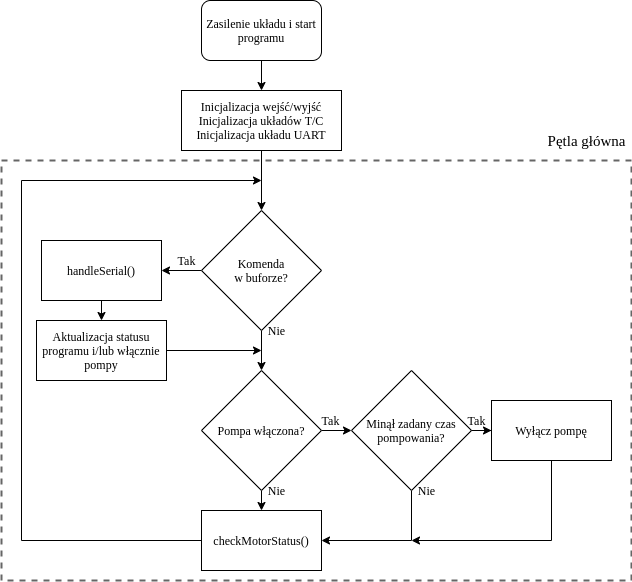
\includegraphics[scale=0.5]{sterownik_schemat}
	\caption{Schemat blokowy programu kontrolera. Źródło: opracowanie własne.} 
	\label{fig:schemat_sterownik}
\end{figure}


\section{Kompilacja sterownika i programowanie układu}

Z uwagi na małą złożoność struktury plików sterownika nie zdecydowano się na użycie narzędzi budowy projektów takich jak CMake. W ramach ułatwienia procesu kompilacji oraz programowania układu, napisano prosty plik reguł Makefile. W pliku tym zawarto trzy reguły:
\begin{itemize}
	\item all: reguła odpowiedzialna za kompilację kodu źródłowego do pliku binarnego .hex
	\item install: reguła odpowiedzialna za zaprogramowanie układu z użyciem pliku .hex i programatora USBASP
	\item clean: metoda usuwająca pliki pośredniczące w procesie kompilacji
\end{itemize}
Taki zestaw reguł okazał się całkowicie wystarczający w procesie rozwoju programu, oraz pozwala nawet osobie bez specjalnej wiedzy na samodzielne zaprogramowanie układu. Projekt można skompilować na każdym systemie z zainstalowanym kompilatorem \textbf{avr-gcc} oraz narzędziem \textbf{avrdude}.

\begin{lstlisting}[caption=Makefile sterownika]

CC=avr-gcc
CFLAGS= -Os -DF_CPU=16000000UL -mmcu=atmega32u4

all: clinostat-stepper-driver.out
%.out: %.cpp
	$(CC) $(CFLAGS) **.cpp -o $@
%.hex: %.out
	avr-objcopy -O ihex -R .eeprom $< $@

install.%: %.hex
	avrdude -F -V -c usbasp -p m32u4 -b 115200 -U flash:w:$<

clean:
	rm -f *.out

\end{lstlisting}
